\documentclass[aspectratio=169, bigger, xcolor=table]{beamer}
\usepackage[magyar]{babel}
\usepackage{t1enc}
\usepackage{lipsum}

\setbeamercovered{transparent}

\begin{document}

    \begin{frame}
        \title{Cím dia}
        \subtitle{Cím dia alcíme}
        
        \maketitle
    \end{frame}

    \begin{frame}{Blokkok}
        \begin{block}
            cím nélkül
        \end{block}
        
        \pause
        
        \begin{block}{sima}
            kék
        \end{block}
        
        \pause
        
        \begin{exampleblock}{példa}
            zöld
        \end{exampleblock}
        
        \pause
        
        \begin{alertblock}{figyelmeztető}
            piros
        \end{alertblock}
    \end{frame}
    
    \begin{frame}{Frame Title}
        \transduration{2}
        \begin{itemize}
            \item<3-> első
            \item<2-> második
            \item<1-> harmadik
        \end{itemize}
    \end{frame}
    
    \begin{frame}{Onslide}
        \begin{theorem}
            Pitagorasz tétele...
        \end{theorem}
        
        \onslide<2>{\begin{proof}[Pitagorasz tétel bizonyítása]
            Készítsünk két darab... \qedhere
        \end{proof}}
    \end{frame}
    
    \begin{frame}{Only}
        \begin{theorem}
            Pitagorasz tétele...
        \end{theorem}
        
        \only<2>{\begin{proof}[Pitagorasz tétel bizonyítása]
            Készítsünk két darab... \qedhere
        \end{proof}}
    \end{frame}
    
    \begin{frame}{Visible}
        \begin{theorem}
            Pitagorasz tétele...
        \end{theorem}
        
        \visible<2>{\begin{proof}[Pitagorasz tétel bizonyítása]
            Készítsünk két darab... \qedhere
        \end{proof}}
    \end{frame}
    
    \begin{frame}{Cím}{Alcím}
        \begin{columns}[t]
            \begin{column}{.5\linewidth}
                \begin{itemize}
                    \item pont
                    \item pontpont
                \end{itemize}
                
                \begin{enumerate}
                    \item első
                    \item második
                    \item harmadik
                \end{enumerate}
            \end{column}
            
            \begin{column}{.5\linewidth}
            \only<1>{\begin{figure}
                    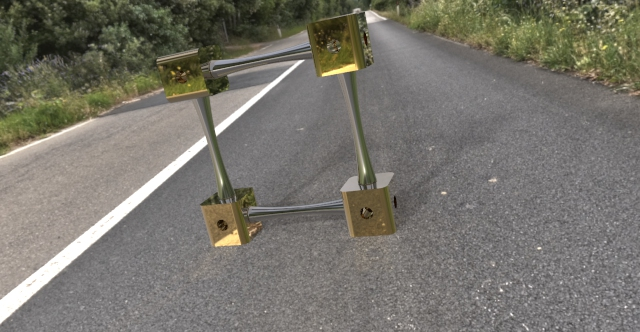
\includegraphics[keepaspectratio, width=5cm]{8. Lesson/creo.jpg}
                    \caption{Kép1}
                \end{figure}}
            \transfade 
            \only<2>{\begin{figure}
                    
\includegraphics[keepaspectratio, width=5cm]{8. Lesson/diagram.jpg}
                    \caption{Kép2}
                \end{figure}}
            \end{column}
        \end{columns}
    \end{frame}
    
\end{document}